Wang et al. \cite{wangDisentanglingLightFields2023} propose the light field disentanglement mechanism,
for processing light field images.
The light field disentanglement mechanism is composed of a spatial, angular and two epipolar feature extractors,
these work along different $2$d subspaces of the $4$d light field and gather complementary information from it.
The model scores the best PSNR and SSIM compared to other state of the art methods for light field super resolution.
Moreover, Wang et al. \cite{wangDisentanglingLightFields2023} report in their ablation study,
that by replacing the Disentanglement Blocks (\ref{eq:distgBlock}) 
by $4$d convolutional residual blocks no improvement could be achieved.
The architecture is visualized in figure \ref{fig:distg}.

\begin{figure}[h!]
    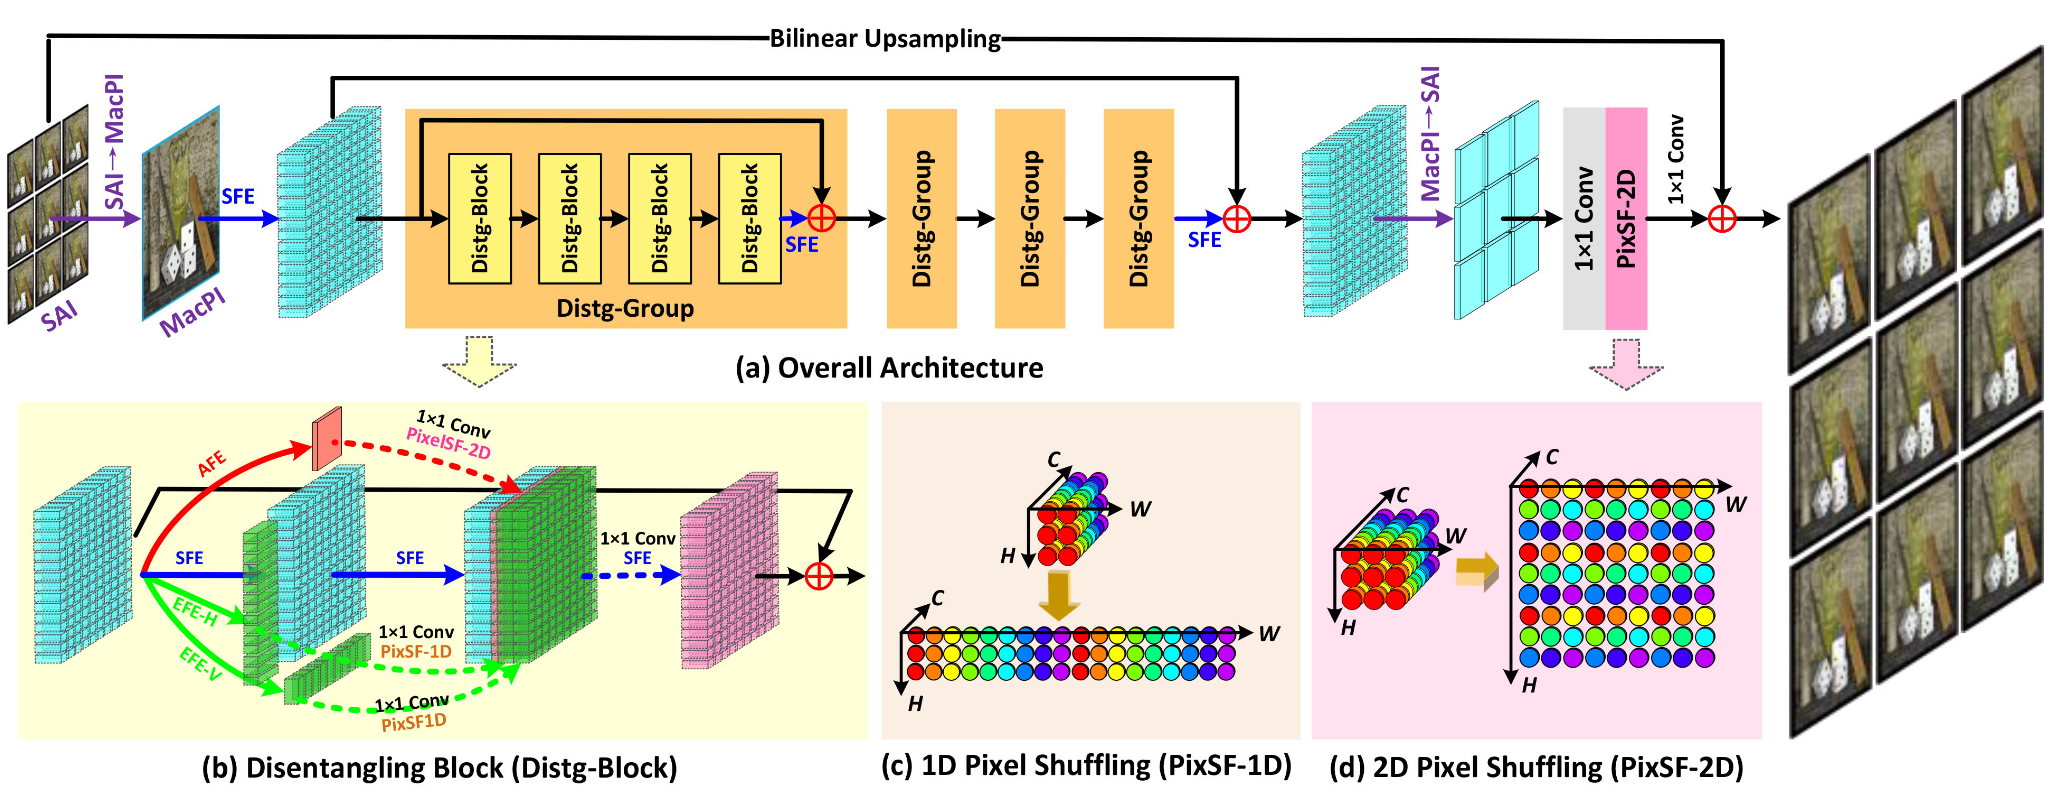
\includegraphics[width=0.9\textwidth]{models/lfsr/imgs/distg.png}
    \caption{Image taken from \cite{wangDisentanglingLightFields2023}.}
    \label{fig:distg}
\end{figure}

Inputs $X \in \mathbb R^{C \times U \times V \times H \times W}$ are reshaped to $C \times HU \times WV$, i.e.

    \begin{equation}
        \label{eq:macpiplane}
        X'(c, h\cdot U + u, w \cdot V + v) = X(c, u, v, h, w) ~, 
    \end{equation}

for $c = 1, ..., C$, $u = 1, ..., U$, $v = 1, ..., V$, $h = 1, ..., H$ and $w = 1, ..., W$,
so that the macro pixels form tiles in a 2d plane.
In the following we are going to assume that the angular dimensions are the same,
i.e. $U = V = A$ for some $A \in \mathbb N$.
The spatial feature extractor only incorporates information belonging to the same SAIs,
to this end a convolution with dilation set to $A$ is employed

\begin{equation}
    \label{eq:sfe}
    C_{sfe} = C(64, 64, \text{kernel-size}=3, \text{padding}=A, \text{dilation}=A, \text{stride}=1) ~.
\end{equation}

The spatial feature extraction module is composed of two spatial feature extractors,
with the leaky ReLU activation function in between 

\begin{equation}
    H_{sfe} = C_{sfe} \circ \text{LReLU}(0.1) \circ C_{sfe} ~.
\end{equation}

The angular feature extractor gathers information only from the same MacPi,
this is achieved by using quadratic kernel of size $A$, i.e. the size of the MacPi itself
and stride set to $A$ 

\begin{equation}
    \label{eq:sfe}
    C_{afe} = C(64, 64, \text{kernel-size}=A, \text{padding}=0, \text{dilation}=1, \text{stride}=A) ~.
\end{equation}

The feature extraction module makes use of only a single angular feature extraction,
due to the stride of $A$ the resulting feature map shrinks by a factor of $A$.
To scale the feature map back to the same size as that produced by $H_{sfe}$ pixel shuffling is employed

\begin{equation}
    H_{afe} = \text{PixelShuffle2D}(A) \circ C(16, A^2\cdot 16, 1) \circ \text{LReLU}(0.1) \circ C_{afe} ~.
\end{equation}

Note that when MacPis are tiled in a $2$d plane as done by the operation described in (\ref{eq:macpiplane}),
the epipolar lines are exactly the rows and the columns.
Hence for epipolar feature extraction a convolution with a kernel of shape $1 \times A^2$ is used,
with a vertical stride of $1$ and a horizontal stride of $A$, padding of $\left \lfloor \frac{A(A-1)}{2} \right \rfloor$
is added to all sides

\begin{equation}
    \label{eq:sfe}
    C_{efe} = C(64, 64, \text{kernel-size}=(1, A^2), \text{padding}=(0, \left \lfloor \frac{A(A-1)}{2} \right \rfloor), \text{dilation}=A, \text{stride}=A) ~.
\end{equation}

Similarly to the angular feature extraction module $H_{afe}$ after the application of the epipolar feature extractor
the feature map needs to be scaled up again

\begin{equation}
    H_{efe} = \text{PixelShuffle1D}(A) \circ C(32, A  \cdot 32, 1) \circ \text{LReLU}(0.1) \circ C_{efe}
\end{equation}

Note that by transposing the input image, $H_{efe}$ can be used to extract features along the vertial epipolar lines.
The Disentanglement Block $H_{Distg}$, shown in part (b) of figure \ref{fig:distg}, forms the basic building block of the architecture proposed by Wang et al. \cite{wangDisentanglingLightFields2023}.
The input is processed in parallel by the spatial, angular and epipolar feature extractors,
the outputs are concatenated and fused by convolution with kernel size $1$ followed by a spatial feature extractor

\begin{equation}
    \label{eq:distgBlock}
    H_{Distg} = R(C_{sfe} \circ C(144, 64, \text{kernel-size}=1) \circ P(H_{sfe}, H_{afe}, H_{efe}, H_{efe} \circ P_\sigma))
\end{equation}

where $\sigma = (1, 3, 2)$.
The deep feature extraction model is composed of $4$ cascaded disentanglement blocks followed by a final spatial feature extraction

    $$ H_d = C_{sfe} \circ H_{Distg} \circ ... \circ H_{Distg} ~. $$